% =====================================================================
% CHAPTERS 4 AND 5
% =====================================================================

\chapter{System Architecture, Data Design and Engineering Decisions}

\section{Architectural Alternatives Evaluated}
At Preliminary Design Review (PDR), three candidate software architectures were evaluated against \texttt{NFR-01}--\texttt{NFR-06}:
\begin{enumerate}
  \item \textbf{Alternative A (Dense DataFrame Procedural Functions)}: Wraps functions operating on dense pandas DataFrames (mirroring \texttt{mlxtend}). Rejected because $\mathcal{O}(N \times M)$ materialization fails on sparse high-cardinality logs ($40.9$~GB on Kosarak) and violates \texttt{scikit-learn} \texttt{Pipeline} interoperability.
  \item \textbf{Alternative B (Subprocess Wrapper Around External Java SPMF)}: Serializes transactions to disk and invokes compiled Java~21 binaries. Rejected because subprocess file I/O incurs $0.4$--$2.5$~s JVM startup overhead, loses \texttt{sample\_\protect\allowbreak{}weight} arithmetic and \texttt{scikit-learn} \texttt{clone()} state, and breaks Python-native pipeline composition.
  \item \textbf{Alternative C (Selected --- Unified Sparse CSR Pipeline with Tri-Engine Core \& Safety Governor)}: Converts raw transactions once via \texttt{TransactionEncoder} into a canonical SciPy CSR matrix shared across Apriori, FP-Growth, and Eclat inside \texttt{Association\protect\allowbreak{}Rules\protect\allowbreak{}Estimator}, governed by \texttt{PruningPolicy}. Selected for sparse scalability, exact parity ($\Delta_{\mathrm{supp}}=0.0$), and fail-safe degradation.
\end{enumerate}

\section{Context View and Trust Boundaries}
External callers (Python scripts, \texttt{Pipeline} stages, CLI operators) cross a strict input-validation trust boundary into \texttt{Association\protect\allowbreak{}Rules\protect\allowbreak{}Estimator.fit(X, sample\_\protect\allowbreak{}weight)} and \texttt{TransactionEncoder.transform(X)}. Only validated binary sparse/dense matrices and non-negative finite weight vectors enter the core mining kernel; continuous floats, NaN/Inf tokens, and invalid thresholds are intercepted immediately before allocation.

\section{Five-Layer Component View and O1--O5 Ownership}
Figure~\ref{fig:ch4_arch} depicts the five-layer architecture of \skarm, mapping component ownership directly across Objectives~\texttt{O1}--\texttt{O5}:
\begin{itemize}
  \item \textbf{Layer 1 --- Sparse Ingestion \& Normalization (\texttt{O1}, \texttt{O4})}: \texttt{datasets.py} ingests CSV, FIMI, and SPMF formats; module \texttt{preprocessing.py} (\texttt{TransactionEncoder}) tokenizes, deduplicates intra-row items idempotently (\texttt{NT-2}), and emits sorted-index boolean SciPy CSR matrices.
  \item \textbf{Layer 2 --- \texttt{scikit-learn} Estimator Contract (\texttt{O4})}: \texttt{Association\protect\allowbreak{}Rules\protect\allowbreak{}Estimator} implements \texttt{BaseEstimator} and \texttt{TransformerMixin}, providing automatic density-based dispatch (\texttt{algorithm='auto'}: routes density $\rho \le 0.15$ to Eclat and density $> 0.15$ to FP-Growth), binary input validation, and \texttt{pickle}/\texttt{joblib} persistence.
  \item \textbf{Layer 3 --- Bit-Exact Tri-Engine Core (\texttt{O2}, \texttt{O3})}: Level-wise Apriori (\texttt{O2} baseline), accelerated FP-Growth (\texttt{O3}), and vertical bitset Eclat (\texttt{O3}) execute over identical CSR matrices using uniform IEEE-754 support arithmetic ($\mathrm{count}/\sum w_r$).
  \item \textbf{Layer 4 --- Auditable Pruning Governor \& Resource Watchdog (\texttt{O3}, \texttt{O4})}: \texttt{PruningPolicy} enforces \texttt{max\_\protect\allowbreak{}candidates}, \texttt{max\_\protect\allowbreak{}len}, \texttt{max\_\protect\allowbreak{}time\_\protect\allowbreak{}seconds}, and cooperative 10~ms RSS checks (\texttt{MemorySampler}) with explicit \texttt{EXACT}/\texttt{DEGRADED} state tracking.
  \item \textbf{Layer 5 --- Deterministic Rule Generation \& Consumption (\texttt{O2}, \texttt{O4})}: \texttt{rules.py} evaluates six metrics and applies canonical lexicographic sorting before exposing outputs to \texttt{Pipeline}, \texttt{RuleExplorer}, and CLI tools.
\end{itemize}

\begin{figure}[ht!]
\centering
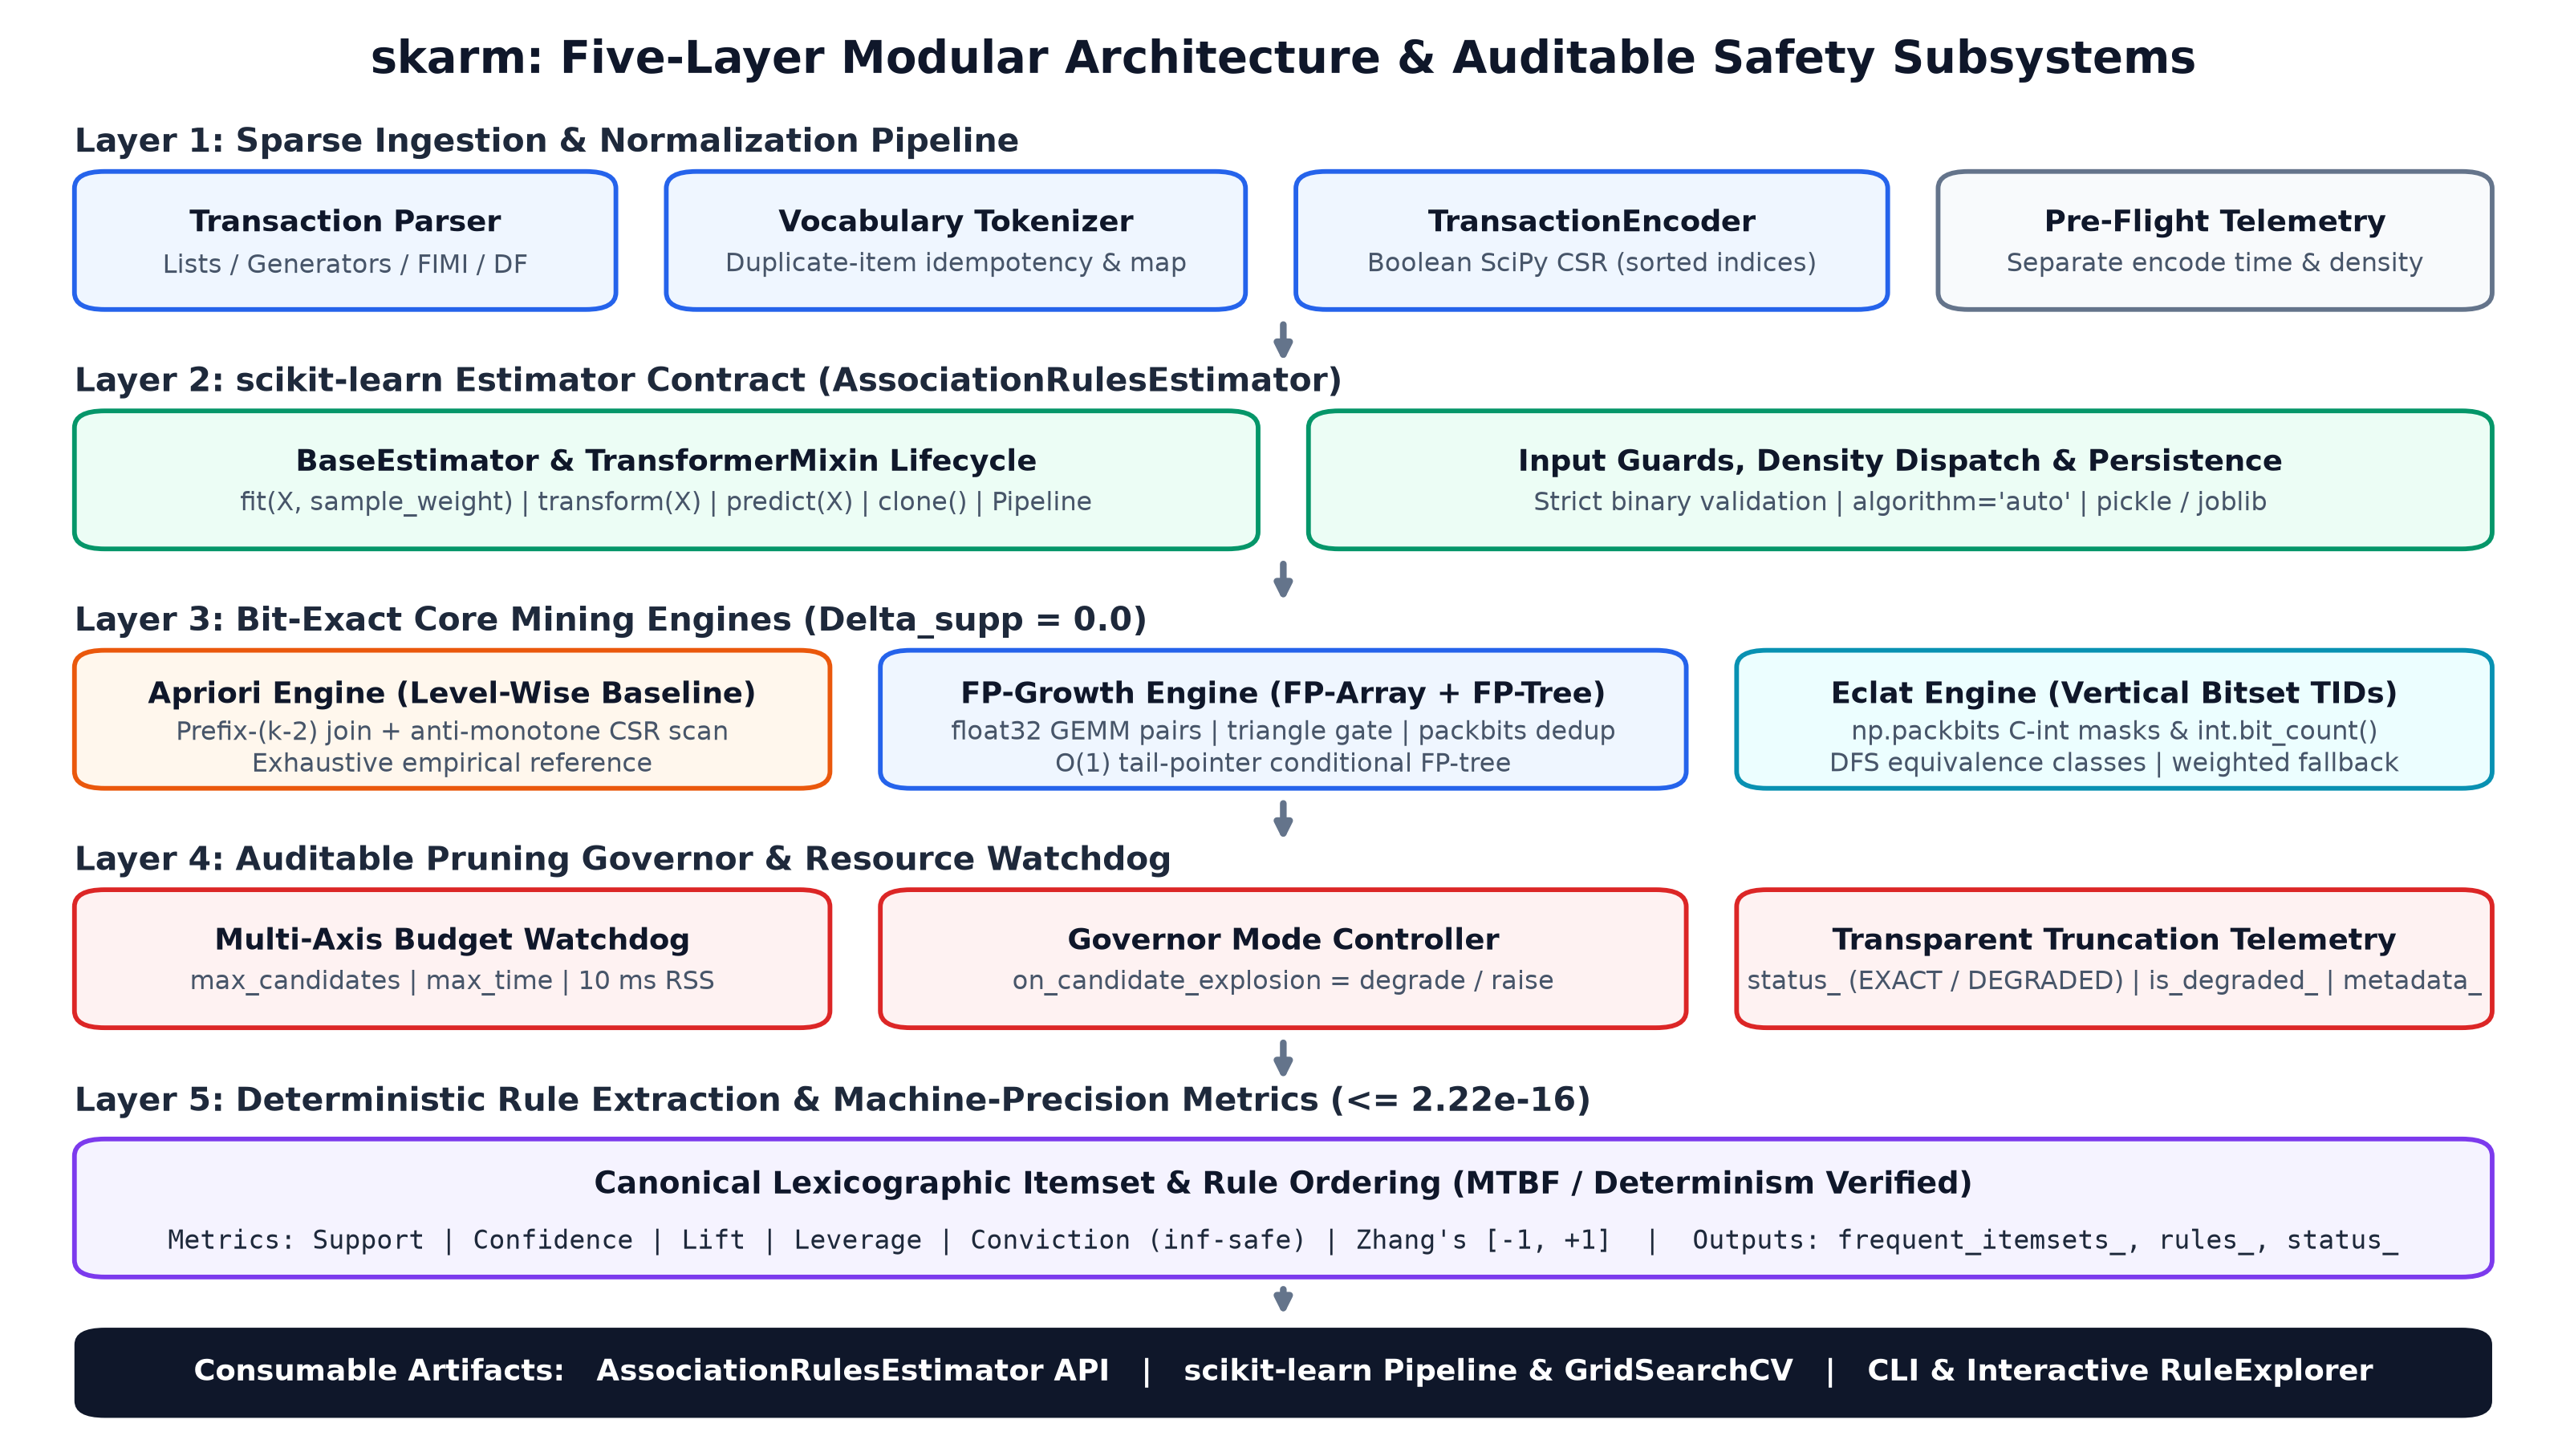
\includegraphics[width=0.86\textwidth,height=0.24\textheight,keepaspectratio]{architecture.png}
\caption{Five-layer modular architecture of \skarm uniting sparse ingestion, estimator lifecycle contracts, three bit-exact miners, cooperative resource governance, and deterministic rule output. Source: Authors' own work.}
\label{fig:ch4_arch}
\end{figure}

\section{Core Mining Engines and Algorithmic Data Structures}
Figure~\ref{fig:ch4_engines} contrasts the execution mechanics of all three mining engines packaged behind \texttt{Association\protect\allowbreak{}Rules\protect\allowbreak{}Estimator}:

\begin{figure}[ht!]
\centering
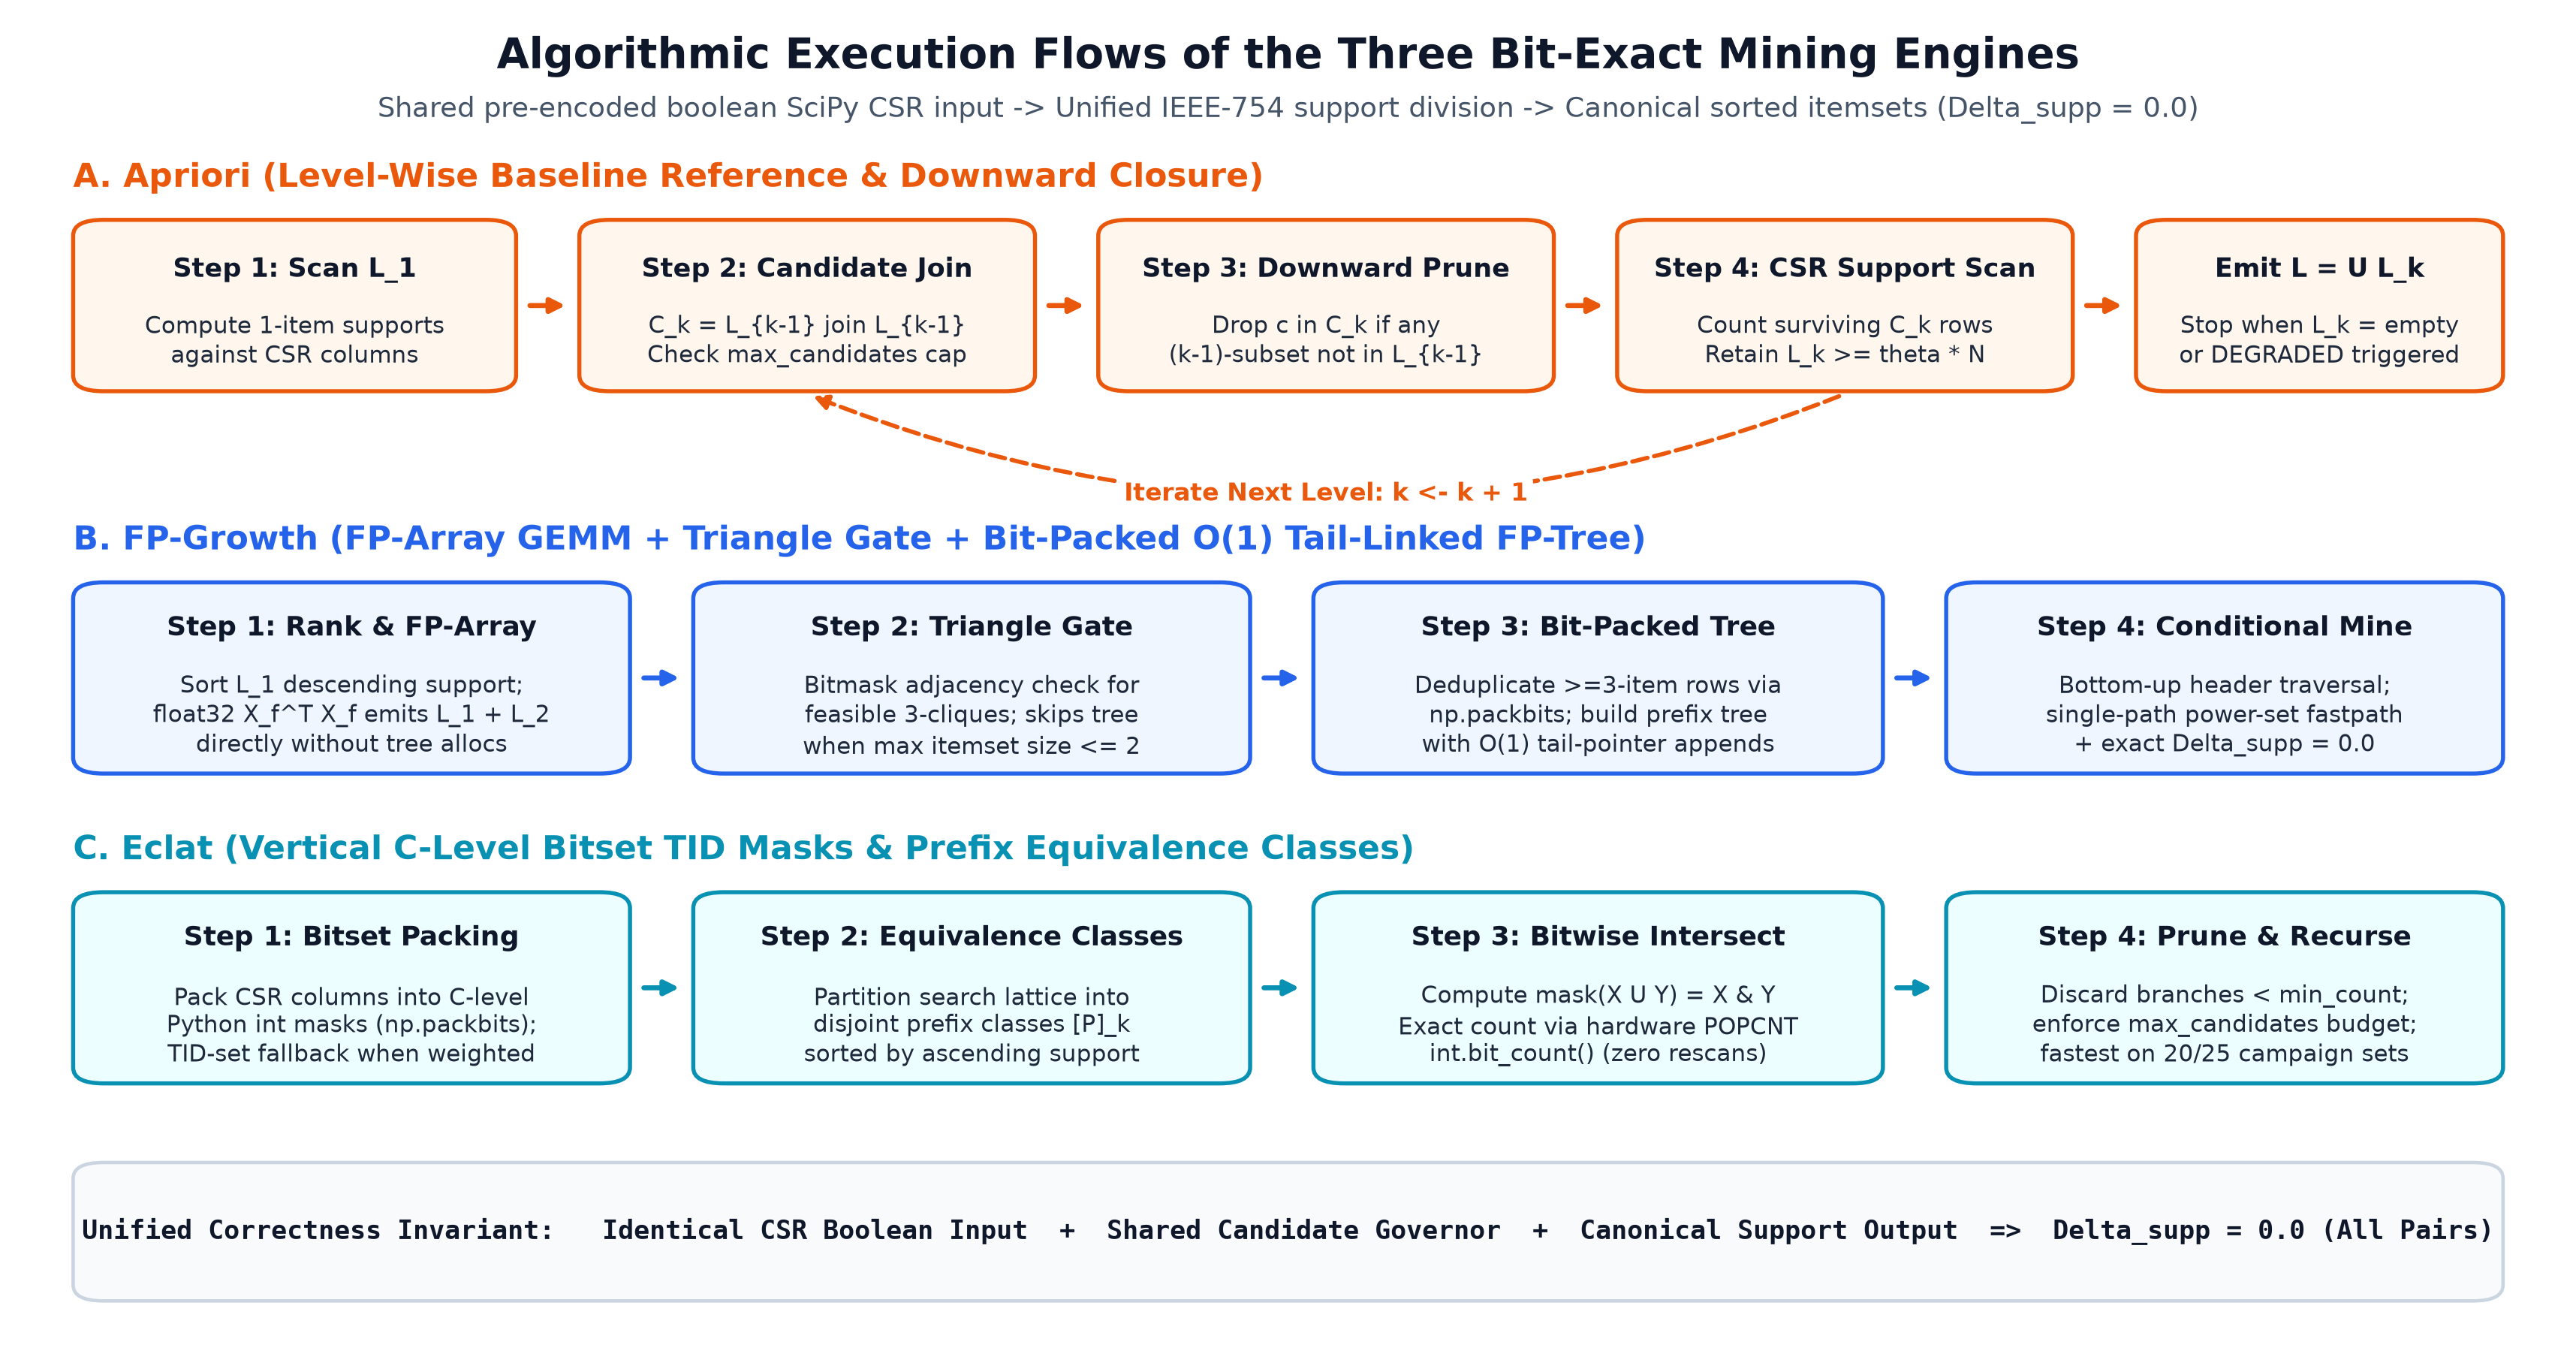
\includegraphics[width=0.86\textwidth,height=0.23\textheight,keepaspectratio]{engines.png}
\caption{Algorithmic execution pipelines of Apriori (reference baseline), FP-Array + $O(1)$ tail-linked FP-Growth, and C-level bitset Eclat behind shared CSR binary inputs. Source: Authors' own work.}
\label{fig:ch4_engines}
\end{figure}

\subsection{Apriori Reference Baseline (\texttt{O2})}
Generates $k$-itemset candidates via $(k-2)$-prefix joins over lexicographically ordered $L_{k-1}$, prunes any candidate whose $(k-1)$-subsets are absent from $L_{k-1}$, and evaluates surviving supports via compressed CSR slices (or weighted row sums). \texttt{skarm/\protect\allowbreak{}apriori.py} remains untouched as the reference baseline across all scaling and correctness regressions.

\subsection{FP-Growth with FP-Array and $O(1)$ Tail-Linked Tree (\texttt{O3})}
To overcome classic Python prefix-tree overhead on both small workloads and sparse clickstreams, \texttt{skarm/\protect\allowbreak{}fpgrowth.py} combines four exact accelerators:
\begin{enumerate}
  \item \textbf{Grahne \& Zhu FP-Array GEMM}: Projects frequent 1-item columns into a chunked \texttt{float32} matrix product $X_f^\top X_f$, emitting exact $L_1$ and $L_2$ counts directly without allocating FP-tree objects.
  \item \textbf{Lossless Triangle \& Depth-3 Gate}: Inspects a pairwise adjacency bitmask for feasible 3-cliques; whenever no 3-clique satisfies $\sigma$, recursion terminates after depth~2 ($L_1 \cup L_2$), bypassing tree construction entirely.
  \item \textbf{Bit-Packed Transaction Compression}: Transactions containing $\ge 3$ frequent items are packed via \texttt{np.packbits} to deduplicate repeated paths with weighted counts prior to tree insertion.
  \item \textbf{Dual-Pointer (\texttt{head} + \texttt{tail}) Header Table}: Canonical FP-tree implementations store only a \texttt{head} link, requiring $\mathcal{O}(L)$ pointer traversal per inserted node and suffering quadratic slowdown on deep clickstream files like BMS-POS. As shown in Figure~\ref{fig:ch4_fptree}, \skarm maintains direct \texttt{tail} pointers per item, reducing node-link insertion to constant $\mathcal{O}(1)$ time while preserving identical prefix topology.
\end{enumerate}

\begin{figure}[ht!]
\centering
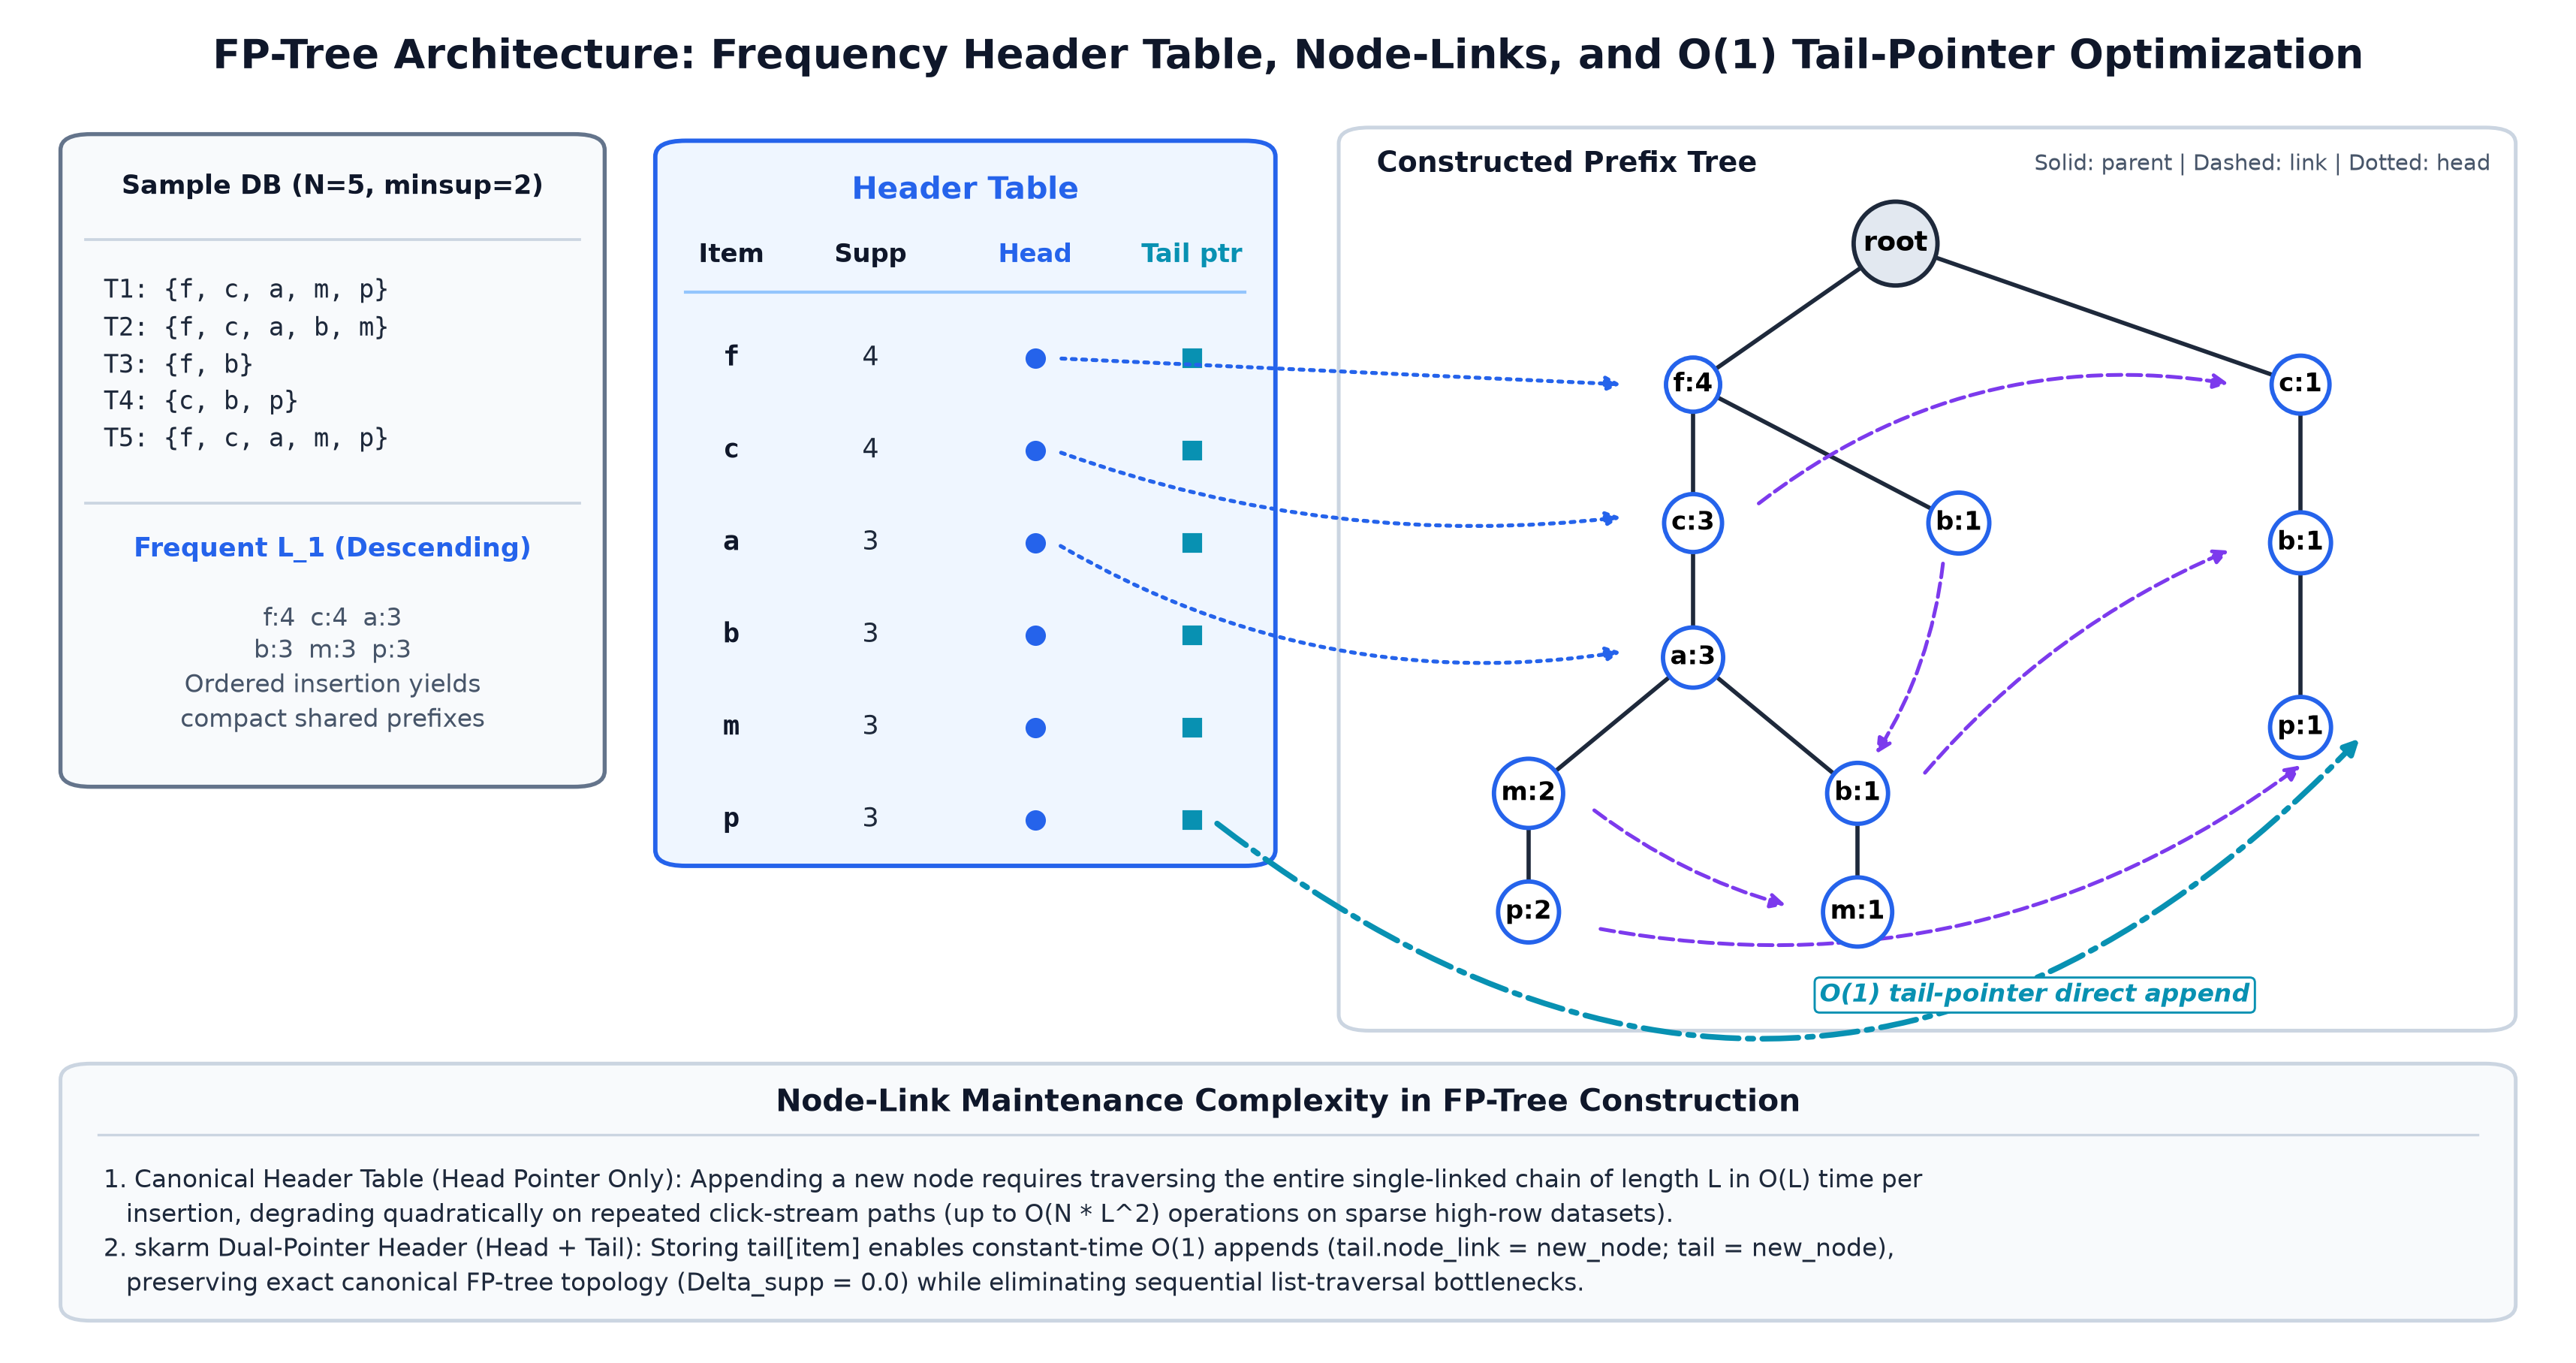
\includegraphics[width=0.84\textwidth,height=0.22\textheight,keepaspectratio]{fptree.png}
\caption{Canonical FP-tree structure (Han \emph{et al.} benchmark database $N=5, \mathrm{minsup}=2$) augmented with \skarm's dual-pointer (\texttt{head} + \texttt{tail}) header table enabling $O(1)$ node-link appends. Source: Authors' own work.}
\label{fig:ch4_fptree}
\end{figure}

\subsection{Vertical C-Level Bitset Eclat (\texttt{O3})}
For unweighted binary matrices, \texttt{skarm/\protect\allowbreak{}eclat.py} packs each frequent column's incidence vector via \texttt{np.packbits} into arbitrary-precision Python integer bitmasks. Prefix equivalence classes $[P]_k$ intersect via bitwise C-level \texttt{\&} and compute support in hardware via \texttt{int.bit\_\protect\allowbreak{}count()} (POPCNT). When transaction weights are provided (\texttt{sample\_\protect\allowbreak{}weight is not None}), Eclat falls back transparently to weighted sparse TID-set intersections, preserving bit-exact parity ($\Delta_{\mathrm{supp}}=0.0$).

\section{Interface Design and Execution Result-State Contract}
To eliminate silent partial failures, every fitted estimator publishes explicit execution telemetry:
\begin{itemize}
  \item \texttt{status\_\protect\allowbreak{}}: Strictly \texttt{'EXACT'} when search completes the full lattice within budgets (\texttt{future\_\protect\allowbreak{}candidates\_\protect\allowbreak{}status='EXHAUSTED'}) or \texttt{'DEGRADED'} when halted by \texttt{max\_\protect\allowbreak{}candidates}, \texttt{max\_\protect\allowbreak{}len}, \texttt{max\_\protect\allowbreak{}time\_\protect\allowbreak{}seconds}, or \texttt{max\_\protect\allowbreak{}memory\_\protect\allowbreak{}mb} (\texttt{future\_\protect\allowbreak{}candidates\_\protect\allowbreak{}status='UNKNOWN'}).
  \item \texttt{is\_\protect\allowbreak{}degraded\_\protect\allowbreak{}}: Boolean flag (\texttt{False} for exact, \texttt{True} when truncated).
  \item \texttt{termination\_\protect\allowbreak{}reason\_\protect\allowbreak{}} and \texttt{metadata\_\protect\allowbreak{}}: Captures \texttt{level\_\protect\allowbreak{}halted}, \texttt{candidates\_\protect\allowbreak{}generated\_\protect\allowbreak{}at\_\protect\allowbreak{}level}, \texttt{peak\_\protect\allowbreak{}candidates}, and operational counters (\texttt{joins\_\protect\allowbreak{}attempted}, \texttt{trees\_\protect\allowbreak{}constructed}, \texttt{intersections\_\protect\allowbreak{}performed}).
\end{itemize}

\section{Data Architecture, Lifecycle and Lineage}
Input transactions flow linearly through four immutable stages without mutating caller buffers (\texttt{check\_\protect\allowbreak{}dont\_\protect\allowbreak{}overwrite\_\protect\allowbreak{}parameters} invariant): raw iterable/DataFrame $\to$ lexicographically mapped vocabulary (\texttt{columns\_\protect\allowbreak{}}) $\to$ boolean SciPy CSR sparse matrix ($X \in \{0,1\}^{N \times M}$) $\to$ canonical sorted \texttt{frozenset} supports and immutable metric DataFrames. Every dataset in \texttt{data/\protect\allowbreak{}} carries recorded provenance, access date (\texttt{2026-10-29}), and measured file metrics in \texttt{DATASET\_\protect\allowbreak{}INVENTORY.md}.

\section{Cooperative Pruning Governor and Resource Safety Design}
Whenever candidate counts exceed \texttt{max\_\protect\allowbreak{}candidates}, runtime exceeds \texttt{max\_\protect\allowbreak{}time\_\protect\allowbreak{}seconds}, or background 10~ms RSS polling (\texttt{MemorySampler}, active when \texttt{max\_\protect\allowbreak{}memory\_\protect\allowbreak{}mb} is configured) crosses the ceiling:
\begin{itemize}
  \item If \texttt{on\_\protect\allowbreak{}candidate\_\protect\allowbreak{}explosion='raise'}, \skarm raises \texttt{Candidate\protect\allowbreak{}Explosion\protect\allowbreak{}Error} cleanly.
  \item If \texttt{on\_\protect\allowbreak{}candidate\_\protect\allowbreak{}explosion='degrade'} (default), \texttt{PruningPolicy} halts deeper exploration (or truncates combinatorial rule expansion), emits \texttt{DegradedModeWarning}, marks \texttt{is\_\protect\allowbreak{}degraded\_\protect\allowbreak{}=True}, and returns all validated patterns discovered up to the safe boundary.
\end{itemize}
As documented transparently in Chapter~3 and Deliverable~D4, this cooperative application-level watchdog guards against runaway loops without replacing OS-level cgroup or container hard limits against instantaneous sub-10~ms allocations.

\section{Security, Input Guards and Deterministic Ordering}
\texttt{rules.py} sorts frequent itemsets and derived rules deterministically by \texttt{(-support, -confidence, -lift, sorted(antecedent), sorted(consequent))}, preventing platform-dependent hash-seed ordering noise across runs (\texttt{NT-5}). Six rule metrics adhere to Hahsler's edge-case conventions \cite{hahsler}: confidence $=1.0$ when antecedent and union supports coincide; conviction returns $+\infty$ rather than raising \texttt{ZeroDivisionError} when confidence $=1.0$; Zhang's metric returns $0.0$ cleanly when independence numerator or denominator vanishes within $10^{-12}$.

\section{Architecture Decision Records (\texttt{ADR-01}--\texttt{ADR-06}) and PDR/CDR Evolution}
Table~\ref{tab:ch4_adrs} summarizes six material architectural decisions (expanded in Appendix~E Template~K). Between Semester~VII PDR and Semester~VIII CDR/Final Defence, two approved refinements occurred: (1)~adding the $O(1)$ tail-pointer header optimization in \texttt{fpgrowth.py} to resolve deep-tree quadratic slowdown on BMS-POS; and (2)~adding the FP-Array + triangle gate + \texttt{np.packbits} bitset Eclat accelerators in \texttt{HEAD} (verified bit-exact at $\Delta_{\mathrm{supp}}=0.0$) while freezing \texttt{apriori.py} and removing small-runtime harness exemptions.

\begin{table}[ht!]
\centering
\caption{Summary of Key Architecture Decision Records (\texttt{ADR-01} to \texttt{ADR-06}).}
\label{tab:ch4_adrs}
\fontsize{9}{11.8}\selectfont
\resizebox{\textwidth}{!}{%
\begin{tabular}{|p{0.11\textwidth}|p{0.25\textwidth}|p{0.34\textwidth}|p{0.22\textwidth}|}
\hline
\textbf{ADR ID} & \textbf{Decision Topic} & \textbf{Selected Option \& Rationale} & \textbf{Evidence Link} \\
\hline
\textbf{ADR-01} & Repository positioning & Standalone \texttt{scikit-learn}-compatible library per \#32712 closure & \texttt{estimator.py} \\
\hline
\textbf{ADR-02} & Canonical matrix format & SciPy boolean CSR sparse representation shared across all 3 engines & \texttt{pre\protect\allowbreak{}processing.py} \\
\hline
\textbf{ADR-03} & Combinatorial safety & Multi-axis \texttt{PruningPolicy} with explicit \texttt{EXACT}/\texttt{DEGRADED} state & \texttt{pruning.py} \\
\hline
\textbf{ADR-04} & Unsupervised contract & Reject non-binary floats (\texttt{Boundary\protect\allowbreak{}Condition\protect\allowbreak{}Error}) rather than silent binarization & \texttt{test\_\protect\allowbreak{}check\_\protect\allowbreak{}estimator} \\
\hline
\textbf{ADR-05} & Deep-tree \& small-scale speedup & Dual \texttt{head/\protect\allowbreak{}tail} links + FP-Array GEMM + \texttt{np.packbits} bitset Eclat & \texttt{fpgrowth.py}, \texttt{eclat.py} \\
\hline
\textbf{ADR-06} & Zero-exemption KPI gate & Remove microbenchmark exemptions; enforce strict 30-trial p95 $\le 0.80\times$ & \texttt{run\_\protect\allowbreak{}acceptance.py} \\
\hline
\end{tabular}}
\end{table}

% =====================================================================
% CHAPTER 5
% =====================================================================
\chapter{System Implementation, Integration and Deployment}

\section{Repository Structure and O1--O5 Module Map}
The implemented codebase resides in \url{https://github.com/ABHISHEK1139/capstone} (\texttt{main} branch, release \texttt{v0.1.0}). Table~\ref{tab:ch5_modules} maps all 13 Python modules inside \texttt{skarm/\protect\allowbreak{}} directly to their verified line counts and \texttt{O1}--\texttt{O5} responsibilities.

\begin{table}[ht!]
\centering
\caption{Source Module Inventory Mapped to Objectives \texttt{O1}--\texttt{O5}.}
\label{tab:ch5_modules}
\fontsize{9}{11.5}\selectfont
\resizebox{\textwidth}{!}{%
\begin{tabular}{|p{0.28\textwidth}|r|p{0.10\textwidth}|p{0.48\textwidth}|}
\hline
\textbf{Module Path} & \textbf{LOC} & \textbf{Obj.} & \textbf{Implemented Subsystem Responsibility} \\
\hline
\texttt{skarm/\_\protect\allowbreak{}\_\protect\allowbreak{}init\_\protect\allowbreak{}\_\protect\allowbreak{}.py} & 56 & O4 & Package exports and version metadata (\texttt{0.1.0}) \\
\hline
\texttt{skarm/\protect\allowbreak{}datasets.py} & 160 & O1, O5 & Unified parsers for FIMI \texttt{.dat}, SPMF \texttt{.txt}, Groceries CSV, header filtering \\
\hline
\texttt{skarm/\protect\allowbreak{}pre\protect\allowbreak{}processing.py} & 227 & O1, O4 & \texttt{TransactionEncoder} (sorted-index CSR / dense ndarray, duplicate idempotency) \\
\hline
\texttt{skarm/\protect\allowbreak{}apriori.py} & 320 & O2 & Untouched level-wise Apriori reference baseline with prefix-$(k-2)$ join \\
\hline
\texttt{skarm/\protect\allowbreak{}fpgrowth.py} & 681 & O3 & FP-Array float32 GEMM, triangle gate, bit-packed dedup, $O(1)$ tail-linked tree \\
\hline
\texttt{skarm/\protect\allowbreak{}eclat.py} & 437 & O3 & C-level \texttt{np.packbits} bitset TID masks (\texttt{int.bit\_\protect\allowbreak{}count()}) + weighted TID fallback \\
\hline
\texttt{skarm/\protect\allowbreak{}pruning.py} & 354 & O3, O4 & \texttt{PruningPolicy}, 10~ms \texttt{MemorySampler}, exception \& warning classes \\
\hline
\texttt{skarm/\protect\allowbreak{}rules.py} & 232 & O2, O4 & Deterministic association rule generation \& 6 machine-precision metrics \\
\hline
\texttt{skarm/\protect\allowbreak{}metrics.py} & 121 & O4 & \texttt{GridSearchCV}-compatible unsupervised scorers (\texttt{mean\_\protect\allowbreak{}confidence\_\protect\allowbreak{}scorer}, etc.) \\
\hline
\texttt{skarm/\protect\allowbreak{}estimator.py} & 529 & O4 & \texttt{Association\protect\allowbreak{}Rules\protect\allowbreak{}Estimator} (\texttt{fit}, \texttt{transform}, \texttt{predict}, auto-dispatch) \\
\hline
\texttt{skarm/\protect\allowbreak{}explorer.py} & 113 & O4 & Interactive \texttt{RuleExplorer} summary formatting and rule filtering \\
\hline
\texttt{skarm/\protect\allowbreak{}telemetry.py} & 85 & O4, O5 & \texttt{TelemetryLogger} and \texttt{RecoveryCoordinator} audit recording \\
\hline
\texttt{skarm/\protect\allowbreak{}cli.py} & 120 & O4 & Command-line runner supporting \texttt{--demo}, \texttt{--dataset}, and \texttt{--algorithm} \\
\hline
\end{tabular}}
\end{table}

\section{Data Preprocessing and Sparse Pipeline Controls}
\texttt{TransactionEncoder} implements \texttt{BaseEstimator} and \texttt{TransformerMixin}, accepting ragged Python lists, sets, or pandas Series/DataFrames. Internally, missing/null items are skipped cleanly (\texttt{\_\protect\allowbreak{}is\_\protect\allowbreak{}missing\_\protect\allowbreak{}token}), unique items are sorted deterministically to freeze \texttt{columns\_\protect\allowbreak{}}, and CSR matrices (\texttt{indptr}, \texttt{indices}, \texttt{data}) are constructed directly with \texttt{bool} dtype without materializing dense $\mathcal{O}(N \times M)$ intermediates. Calling \texttt{fit} or \texttt{fit\_\protect\allowbreak{}transform} guarantees zero duplicate inflation within any transaction (\texttt{['A','A','B']} contributes unit weight once per row).

\section{Core Mining Engines and Metric Derivation}
To ensure numerical consistency without screenshots of code, Listing~\ref{lst:metrics} reproduces the exact verified IEEE-754 metric kernels from \texttt{skarm/\protect\allowbreak{}rules.py} (lines~17--42) used to compute conviction and Zhang's association metric with zero-denominator stability, and Listing~\ref{lst:sampler} shows the on-demand 10~ms RSS watchdog from \texttt{skarm/\protect\allowbreak{}pruning.py} (lines~48--84).

\begin{lstlisting}[caption={Verified Conviction and Zhang's Metric Edge-Case Implementations (\texttt{skarm/rules.py}, lines 17--41).},label={lst:metrics}]
def compute_conviction(supp_c: float, confidence: float) -> float:
    """Compute conviction = (1 - supp(C)) / (1 - confidence)."""
    if math.isclose(confidence, 1.0, abs_tol=1e-12) or confidence >= 1.0:
        return float("inf")
    denom = 1.0 - confidence
    if denom <= 0.0:
        return float("inf")
    return float((1.0 - supp_c) / denom)

def compute_zhangs_metric(supp_ac: float, supp_a: float, supp_c: float) -> float:
    """Compute Zhang's association metric (-1 to +1)."""
    num = supp_ac - (supp_a * supp_c)
    if math.isclose(num, 0.0, abs_tol=1e-12):
        return 0.0
    denom = max(supp_ac * (1.0 - supp_a), supp_a * (supp_c - supp_ac))
    if denom <= 1e-12:
        return 0.0
    val = float(num / denom)
    return float(max(-1.0, min(1.0, val)))
\end{lstlisting}

\section{Pruning Governor, Estimator Integration and CLI Operability}
\begin{lstlisting}[caption={Cooperative 10~ms Background RSS Memory Sampler (\texttt{skarm/pruning.py}, lines 48--84).},label={lst:sampler}]
class MemorySampler(threading.Thread):
    """Continuous background RSS memory sampler (10 ms polling = 100 Hz)."""
    def __init__(self, polling_interval: float = 0.01):
        super().__init__(daemon=True)
        self.polling_interval = polling_interval
        self._stop_event = threading.Event()
        self._lock = threading.Lock()
        self.baseline_mb: float = get_current_memory_mb()
        self._peak_mb: float = self.baseline_mb

    def run(self):
        while not self._stop_event.is_set():
            try:
                curr = get_current_memory_mb()
                with self._lock:
                    if curr > self._peak_mb:
                        self._peak_mb = curr
            except Exception:
                pass
            self._stop_event.wait(self.polling_interval)
\end{lstlisting}

When integrated inside a \texttt{scikit-learn} \texttt{Pipeline}:
\begin{itemize}
  \item \textbf{Terminal Estimator Role}: Accepts sparse CSR output from upstream vectorizers (\texttt{TransactionEncoder}) and produces ranked recommendation predictions via \texttt{predict(X)} (matching antecedent itemsets whose confidence/lift maximize rule firing for each query row).
  \item \textbf{Intermediate Transformer Role}: \texttt{transform(X)} projects rows onto binary rule-activation columns (\texttt{shape=(N, n\_\protect\allowbreak{}rules)}) and implements \texttt{get\_\protect\allowbreak{}feature\_\protect\allowbreak{}names\_\protect\allowbreak{}out()} cleanly for downstream classifiers or regressors (benchmarked in \texttt{benchmarks/pipeline\_\protect\allowbreak{}benchmark.py} and verified in E2E Tier~4).
\end{itemize}

\section{Build Configuration, Dependencies, Licences and CI/CD}
Package distribution metadata and dependencies are locked cleanly via \texttt{requirements.txt} (\texttt{numpy>=1.24.0}, \texttt{scipy>=1.10.0}, \texttt{pandas>=2.0.0}, \texttt{scikit-learn>=1.3.0}, \texttt{joblib>=1.2.0}, \texttt{pytest>=7.0.0}, \texttt{psutil>=5.9.0}), MIT \texttt{LICENSE}, and \texttt{CITATION.cff} (\texttt{v0.1.0}). Continuous Integration (\texttt{.github/\protect\allowbreak{}workflows/\protect\allowbreak{}ci.yml}) triggers automatically on every push and pull request to \texttt{main} across a three-version Python matrix (\texttt{3.10}, \texttt{3.11}, \texttt{3.12}), executing: (1)~\texttt{pytest -v tests/\protect\allowbreak{}} (264 tests); (2)~\texttt{python tests/run\_\protect\allowbreak{}acceptance.py}; and (3)~\texttt{python -m skarm.cli --demo}.

\section{Deployment, Installation and Reproducible Execution Runbook}
Fresh deployment from Git requires only standard virtual-environment setup (\texttt{python -m venv .venv} $\to$ \texttt{pip install -r requirements.txt}). Full dataset restoration runs \texttt{python scripts/download\_\protect\allowbreak{}datasets.py}, and all test/benchmark suites execute cleanly via deterministic scripts summarized in Appendix~D. Known operational limitations match Chapter~10: single-host execution without distributed Spark sharding and strict binary transaction inputs.
